\section{Traffic models and routes}
We wish to determine how well the system complies with criteria \ref{crit:timesaving} and \ref{crit:cost} of the solution criteria in \secref{chap:solutioncriteria} and how the system can alleviate the problem described in the problem statement. To achieve this, we need to evaluate the following:
% What do we look at to evaluate?
\begin{itemize}
\item How accurately does the regression models reflect the actual traffic?
\item Do the routes found based on the regression models reflect reality?
\item Are routes found by the system faster than routes chosen by drivers?
\end{itemize}
% How do we evaluate?
To answer the above questions, we consider the model accuracies and time improvements of the routes. 

The model accuracy is the difference between the predicted traffic of the regression model and the actual traffic. In order to find the model accuracy we consider both the accuracy on a route basis as well as on an waypoint-to-waypoint basis.

Time improvement represent how much faster a found route is than an actual route. This is found by comparing actual routes from a test set of routes and routes found by querying the system the same start and destination.

\subsubsection{Route evaluation}
The following method is used to find the differences between real routes driven as given by the test-set and the routes found by the system.
\begin{enumerate}
\item First, we select a route $R=(n_1,...n_m)$ from the GPS data that originates in $n_1$ and ends in $n_m$. We then, directly from the data, determine the weight (i.e. the travel time) of the route, $W_o(R)$.
\item Secondly, we compute a new weight, $W_{a}(R)$ for every edge $(n_i,n_{i+1}) \  for \  1 \leq i < m$ with the weight function described in \secref{sec:weight-function}.
\item Now, we traverse the road network to find a new route, $R'$ originating in $n_1$ and ending in $n_m$ such that the route is the shortest path (in time) from $n_1$ to $n_m$ by using the weight of each edge determined by the weight function.
\item We compare $W_o(R)$ and $W_a(R)$ to see the total weight difference. This is the \emph{route model accuracy}.
\item Finally, we compare $W_a(R')$ with $W_a(R)$ and find the difference. This is the \emph{time improvement}.
\end{enumerate}
The process is illustrated in the graphs in \figref{fig:eval}. Blue nodes represent start nodes, green nodes represent goal nodes where the number in goal nodes are the aggregate weight of all the edges in the route. 

Red arrows represents the uninformed route $R$, with a total weight of 7. $R$ with adjusted weights, has a total weight of 8. This means that the regression models has a route model accuracy of $\frac{7}{8}=0.875=87.5\%$. 

By computing the informed route $R'$, based on the regression model weights, the route marked with yellow arrows are found. $R'$ has a total weight of 6; a lower weight than $R$. This means that the time improvement is 1.

\begin{figure}
\centering
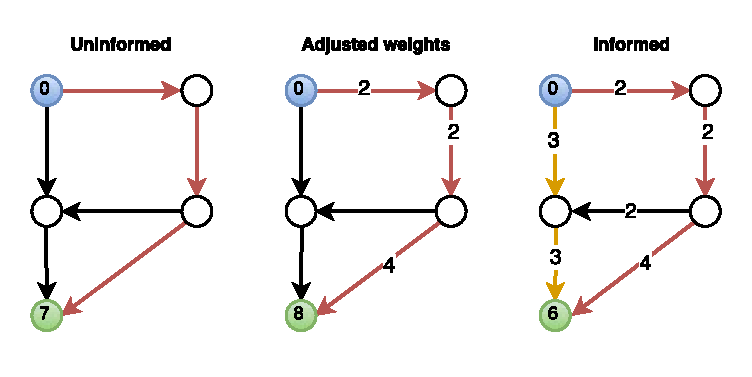
\includegraphics[width=\textwidth]{figures/eval.pdf}
\caption{The evaluation process}
\label{fig:eval}
\end{figure}

We follow the approach on a set of 7 fairly small routes that has no signs of intermediate stops, since intermediate stops in the route, without further measures taken, would skewer the travel time in favour of our system. 
\begin{table}[]
\centering
\begin{tabular}{llllll}
\textbf{Route} & \textbf{$W_o(R)$} & \textbf{$W_a(R)$}  & \textbf{$W_a(R')$} & \textbf{RMA (\%)} & \textbf{TI (\%)} \\ \hline
$r_1$          & 353               & 393                & 263                & 89.8                         & 38.5 \\
$r_2$          & 1822              & 2016               & 1552               & 90.4                         & 20.5 \\
$r_3$          & 1012              & 551                & 250                & 54.4                         & 15.3 \\
$r_4$          & 297               & 322                & 107                & 92.2                         & 43.0 \\
$r_5$          & 1248              & 927                & 797                & 74.3                         & 31.3 \\
$r_6$          & 469               & 440.5              & 440.0              & 93.9                         & 25.2 \\
$r_7$          & 1676              & 1462               & 989                & 87.2                         & 19.4 \\ \hline
mean       	   &                   &                    &                    & 83.2                         & 27.6
\end{tabular}
\caption{RMA = Route Model Accuracy = $100 * \frac{min(W_o(R), W_a(R))}{max(W_o(R), W_a(R))}$\\
	     TI = Time Improvement = $100 * \frac{W_a(R) - W_a(R')}{W_a(R)}$}
\label{tab:eval-results}
\end{table}

\tabref{tab:eval-results} shows the time in seconds, $W_0(R)$, for the uninformed route $R$, the adjusted time, $W_a(R)$, for route $R$, and the informed time $W_a(R')$ for the new (informed) route $R'$.

\emph{Route Model Accuracy } (\textbf{RMA}) represents the difference between the uninformed weight and the adjusted weight. The closer the route model accuracy is to 100\%, the closer the regression models are to represent the actual traffic.
 
\emph{Time Improvement} (\textbf{TI}) represents the time saved for route $r_i$ by traveling the informed route instead of the uninformed route. The higher the time improvement, the better the informed routing is.

The mean route model accuracy, shows that the regression models predicts the traffic within 83.2\% of the actual traffic. 

The mean time improved value shows that for the tested routes, there are on an average time improvement 27.6\% by following the routes used by the system. However, it is worthwhile to note that it is not known if the drivers in the test routes was using some kind of GPS routing or not, which means that it is not possible to tell if the system outperforms routes selected by drivers or other systems. Likewise, the mean route model accuracy in \tabref{tab:eval-results} only shows the aggregate accuracy, which could be misleading if there is a high deviation in the regression model predictions and the actual traffic, throughout the edges. For this reason, the regression model accuracy must also be determined on a smaller basis.

\subsubsection{Waypoint-to-waypoint accuracy}
The smallest part of a route we can observe is a waypoint. The shortest travel times we can find are those between consecutive waypoint pairs. Consequently, the smallest part of a route we can evaluate is travel time on a waypoint-to-waypoint basis. The result is presented in \tabref{tab:eval-results-2}.

\begin{table}[H]
	\centering
	\begin{tabular}{lll}
		\textbf{Route} & \textbf{Mean error (s)}                          & \textbf{Mean accuracy (\%)} \\ \hline
		$r_1$          & 3.66                                             & 39.8 \\
		$r_2$          & 0.722                                            & 68.1 \\
		$r_3$          & 1.61                                             & 50.0 \\
		$r_4$          & 1.69                                             & 46.4 \\
		$r_5$          & 1.13                                             & 59.0 \\
		$r_6$          & 2.70                                             & 40.9 \\
		$r_7$          & 1.01                                             & 57.9 \\ \hline
		mean           & 1.79                                             & 51.7
	\end{tabular}
	\caption{Mean accuracy \% is the mean of the percent errors of each consecutive waypoint pair subtracted from 100\%.}
	\label{tab:eval-results-2}
\end{table}

We start by extracting all the waypoints from each link in the route. As described in \secref{sec:mapmatching}, a link contains zero or more waypoints. We only consider waypoint pairs within each link, i.e. we do not consider inter-link waypoint pairs. Inter-link waypoints are sometimes several ways apart, which means some of the edges between them have to be predicted by the map-matcher, so including them in the evaluation could skew the result.

When we have the waypoints, we go through them one link at a time. For each consecutive waypoint pair, we can find the actual time travelled by looking at the difference in time between them. We then calculate the travel time using our weights by summing the distance travelled on each edge divided it by the weight of the edge. The time used in the weight functions is the start time in the actual route for the first node, and the start time plus the travel time so far for the rest.

The error in seconds for each consecutive waypoint pair can now be calculated as $error = |T_a - T_w|$, where $T_a$ is the actual time travelled, and $T_w$ is the travel time without weights. The error percentage is calculated as $\frac{error}{max(T_a, T_w)}$. The raw evaluation data for the first route can be seen in \appref{app:rawevaldata}.
\\\\
The test set of seven routes might not be representative of the whole dataset, which means that it would be preferable to perform further evaluation on a larger set of routes to get a more precise route model accuracy. Furthermore, it is not possible to know for sure whether the test routes have no intermediate stops, or are driving the route for a reason other than getting from A to B. We have tried to select where that do not exhibit such behaviour. It would have been preferable to perform a number of test drives ourselves and use these as test routes, since this would ensure no intermediate stops and would enable us to directly measure the speed instead of estimating it.

Furthermore, the training set contains data from February 2-8, 2008, while the selected test routes are from August 23, 2009 to November 5, 2009. It would have been preferable to have training data that immediately precedes the test data.
